\documentclass{report}

\usepackage[T1]{fontenc}
\usepackage[polish]{babel}
\usepackage[utf8]{inputenc}
\usepackage{graphicx}
\usepackage{amsmath,amssymb}
\usepackage{makeidx}
\usepackage{acronym}
\usepackage{array}
\usepackage{hyperref}



\title{Malware: Złośliwe oprogramowanie w pigułce\\[0.3cm] \small wersja prezentacji \cite{prezentacja} zmodyfikowana do klasy dokumentu \texttt{report} na potrzeby projeku z kodu LateX}
\author{Cezary Kosowski}
\date{13.04.2026}
\makeindex
\begin{document}
\maketitle
\newpage
\tableofcontents
\listoftables
\listoffigures
\chapter*{Wykaz skrótów}
\addcontentsline{toc}{chapter}{Wykaz skrótów}
\begin{acronym}
    \acro{AI}{Sztuczna Inteligencja (ang. \textit{Artificial Inteligence})}
    \acro{BIOS}{Basic Input/Output System}
    \acro{IT}{Informatyka (ang. \textit{Information Technology}}
    \acro{malware}{złośliwe oprogramowanie (ang. \textit{Malicious software}}
\end{acronym}
\chapter{Wprowadzenie do złośliwego oprogramowania}
\newpage
\section{Informacje ogólne}
\noindent Malware\index{malware} to pojęcie ogólne oznaczające \ac{malware},\\
typy malware to między innymi:
\begin{itemize}
    \item Wirus\index{wirus}
    \item Robak\index{robak}
    \item Ransomware\index{ransomware}
    \item Trojan\index{trojan} \cite{prezentacja}
\end{itemize}
\newpage
\chapter{Analiza wybranych typów Malware}
\newpage
\section{Klasyczny Wirus} 
\begin{table}[htbp]
    \begin{tabular}{|c|m{10cm}|}
    \hline
    \textbf{Cecha} & \textbf{Opis}\\
    \hline
    \textbf{Ogólna zasada} & Działa na podobnych zasadach jak biologiczny wirus.\\
    \hline
    \textbf{Zależność} & Nie jest samodzielnym programem, potrzebuje „żywiciela” – dodaje swój kod do legalnych plików (np. programów, dokumentów).\\
    \hline
    \textbf{Powielanie} & Powiela się samodzielnie, po uruchomieniu zainfekowanego programu wirus się uruchamia i infekuje następne pliki.\\
    \hline
    \textbf{Zadanie} & Jego zadanie to najczęściej niszczenie i modyfikowanie plików lub uszkadzanie systemu operacyjnego.\cite{wirus}\\
    \hline
    \end{tabular}
    \caption{Charakterystyka wirusa komputerowego}
    \label{tab:Klasyczny wirus}
\end{table} 
\begin{figure}[!h]
    \centering
    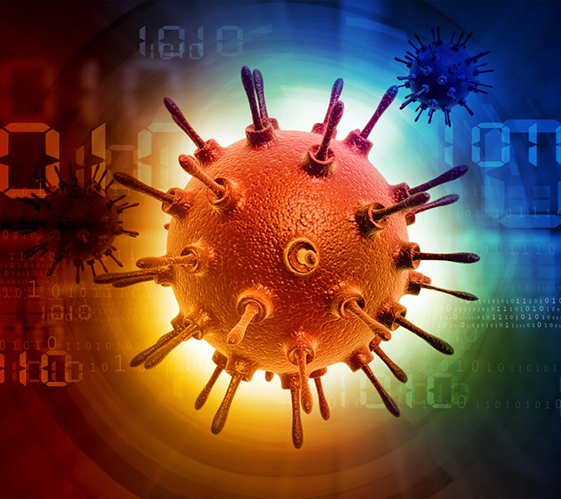
\includegraphics[width=1\linewidth]{wirus_rys.png}
    \caption{Artystyczna wizja wirusa komputerowego \cite{grafiki}}
    \label{wirus}
\end{figure}
\newpage
\subsection{Przykład - CIH ,,Czarnobyl'' \index{Czarnobyl}}
\begin{figure}[!h]
    \centering
    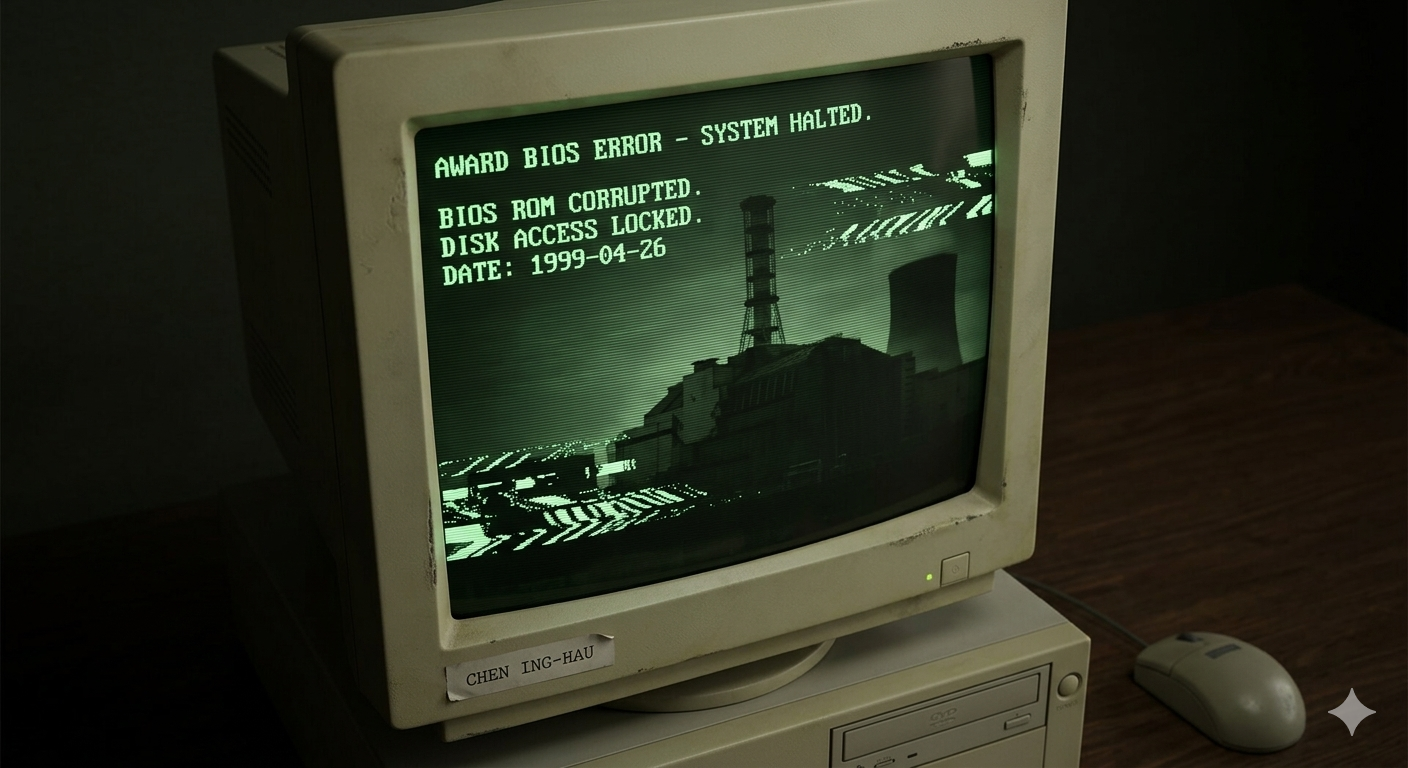
\includegraphics[width=1\linewidth]{czarnobyl.png}
    \caption{Wirus oczami \ac{AI} \cite{grafiki}}
    \label{fig:czarnobyl}
    \index{AI}
\end{figure}
\begin{itemize}
    \item \textbf{Pochodzenie i twórca:} Tajwański student {Chen Ing-Hau}
    \item \textbf{Data ataku:} {26 kwietnia 1999}
    \item \textbf{Metoda Kamuflażu:} {„Spacefiller”}
    \item \textbf{Skutki infekcji:} {Blokada dysku i atak na Bios}
    \item \textbf{Mity:} {Totalne zniszczenie płyty głównej} \cite{wirus_przyklad}
\end{itemize}
\newpage
\section{Robak}
Jaka zaznaczono wcześniej w Tabeli \ref{tab:Klasyczny wirus} na stronie \pageref{tab:Klasyczny wirus}, klasyczny wirus potrzebuje żywiciela. Robak\index{robak} działa zupełnie inaczej:
\begin{itemize}
    \item Jest w pełni samodzielnym programem
    \item Rozprzestrzenia się automatycznie i replikuje przez sieć, bez konieczności działania użytkownika.
    \item Jego głównym celem jest zużywanie zasobów sieciowych lub otwieranie „tylnych furtek” (\textit{backdoor}\index{backdoor}). \cite{robak}
\end{itemize}
\begin{figure}[!h]
    \centering
    \includegraphics[width=1\linewidth]{robak.png}
    \caption{Symboliczna reprezentacja robaka komputerowego przełamującego zabezpieczenia systemu. \cite{grafiki}}
    \label{fig:robak}
\end{figure}
\subsection{Matematyczny model\index{model matematyczny} infekcji}
\begin{equation}
    I(t) = I_0 \cdot e^{rt}
    \label{eq:infekcja}
\end{equation}
Jak wynika ze wzoru \eqref{eq:infekcja}, w którym $I_0$ to początkowa liczba zainfekowanych maszyn, a $r$ to wskaźnik infekcji, liczba zarażonych komputerów rośnie lawinowo w bardzo krótkim czasie. 
\newpage
\subsection{Przykład – Robak Morrisa\index{Robak Morrisa}}
\begin{figure}[!h]
    \centering
    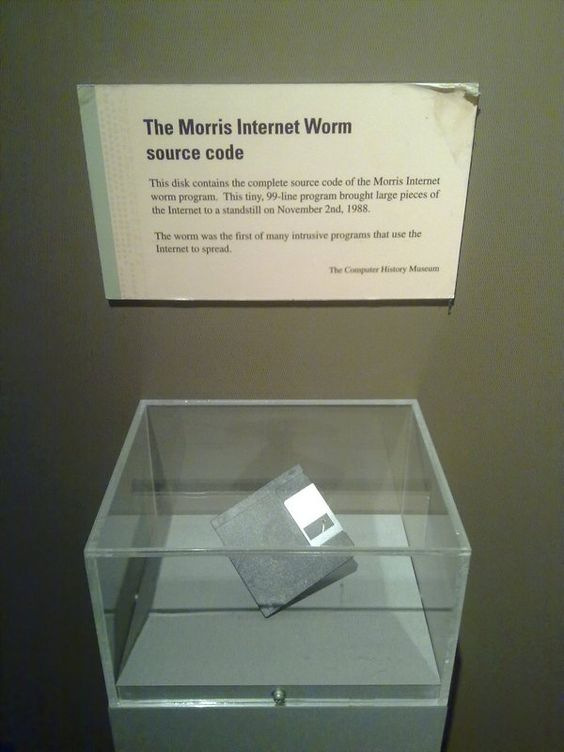
\includegraphics[width=0.5\linewidth]{robak_muzeum.png}
    \caption{Dyskietka z kodem źródłowym w muzeum. \cite{grafiki}}
    \label{fig:robak_muzeum}
\end{figure}
\begin{itemize}
    \item \textbf{Pochodzenie i twórca} Amerykański student Robert Tappan Morris.
    \item \textbf{Data ataku:} 2 listopada 1988 r.
    \item \textbf{Cel:} Niegroźne badanie luk w zabezpieczeniach
    \item \textbf{Skutki infekcji:} Paraliż około 10\% ówczesnego Internetu (ponad 6 tys. komputerów)
    \item \textbf{Konsekwencje dla autora:} Wyrok sądowy \cite{robak_morris}
\end{itemize}
\newpage
\chapter{Zagrożenia współczesne i socjotechnika\index{socjotechnika}}
\newpage
\section{Ransomware}
Złośliwe oprogramowanie, które dosłownie „bierze nasze dane jako zakładników”.
\begin{itemize}
    \item Szyfruje pliki osobiste lub całkowicie blokuje dostęp do systemu (komputera, smartfona)
    \item Głównym celem jest wymuszenie okupu\index{okup} (często płatnego w kryptowalutach) w zamian za przywrócenie dostępu do danych
    \item Do infekcji dochodzi najczęściej poprzez nieostrożność użytkownika (np. kliknięcie w podejrzany załącznik mailowy – \textit{malspam\index{malspam}}, lub fałszywą reklamę – \textit{malvertising \index{malvertising}}) \cite{ransomware}
\end{itemize}
\begin{figure}[!h]
    \centering
    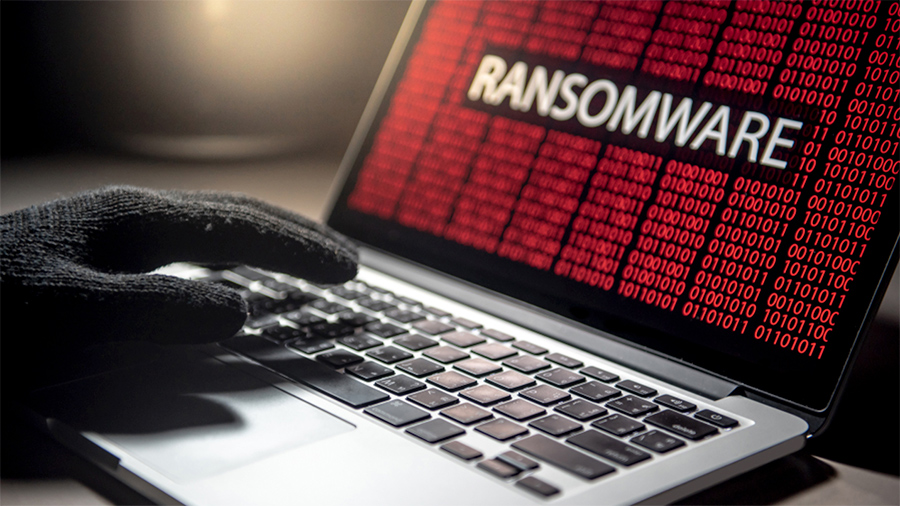
\includegraphics[width=1\linewidth]{ransomware.png}
    \caption{Wizualizacja ataku typu ransomware. \cite{grafiki}}
    \label{fig:ransomware}
\end{figure}
\newpage
\subsection{Przykład-WannaCry\index{WannaCry}}
\begin{figure}[!h]
    \centering
    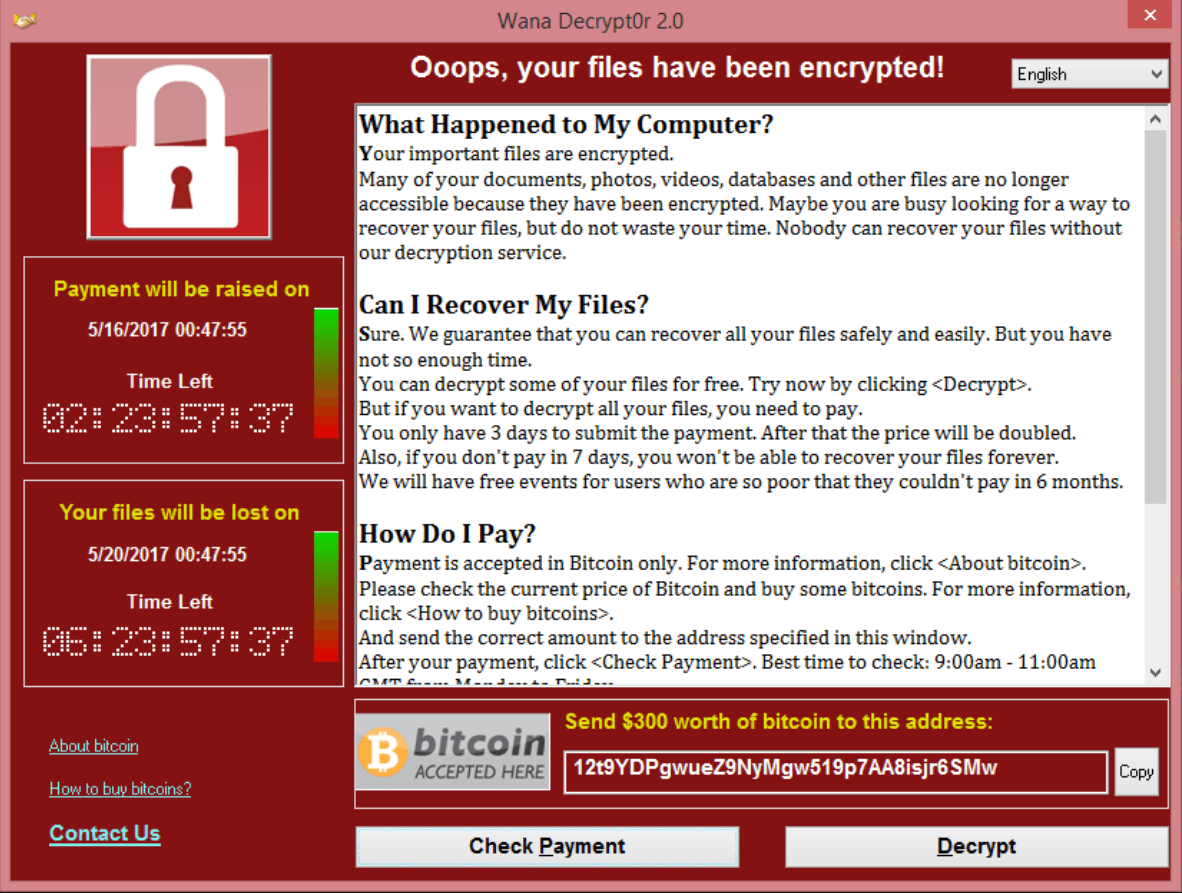
\includegraphics[width=1\linewidth]{Wannacry.png}
    \caption{Komunikat żądanie okupu z ataku WannaCry. \cite{grafiki}}
    \label{fig:WannaCry}
\end{figure}

\noindent Zgodnie z ilustracją \ref{fig:WannaCry}, użytkownik otrzymuje określoną ilość czasu na zapłatę. W przypadku \textbf{WannaCry} atak wykorzystywał lukę w systemach Windows o nazwie \texttt{EternalBlue}.

\begin{itemize}
    \item \textbf{Pochodzenie i twórca:} Nieznany (podejrzenia kierowane w stronę Korei Północnej)
    \item \textbf{Data ataku:} 12 maja 2017
    \item \textbf{Metoda ataku:} Ransomware (szyfrujące) + Robak (wykorzystanie luki „EternalBlue”)
    \item \textbf{Skutki infekcji:} Szyfrowanie\index{szyfrowanie} danych i żądanie okupu, paraliż ponad 230 tys. Komputerów
    \item \textbf{Zatrzymanie:} Odkrycie „wyłącznika awaryjnego” (kill switch) przez brytyjskiego badacza \cite{wannacry}
\end{itemize}
\newpage
\section{Trojan}
Złośliwe oprogramowanie, które podszywa się pod użyteczne i legalne programy.
\begin{itemize}
    \item Ukrywa swoje prawdziwe zamiary pod przykrywką przydatnej aplikacji, licząc na to, że użytkownik sam go zainstaluje.
    \item W przeciwieństwie do wirusów i robaków, trojany zazwyczaj nie replikują się samodzielnie i potrzebują interakcji użytkownika (np. uruchomienia pobranego pliku).
    \item Często służy jako furtka dla innych zagrożeń – kradnie dane (hasła, dane finansowe), szpieguje (\textit{spyware}) lub pobiera kolejne złośliwe programy, np. \textit{ransomware}. \cite{trojan}
\end{itemize}
\begin{figure}[!h]
    \centering
    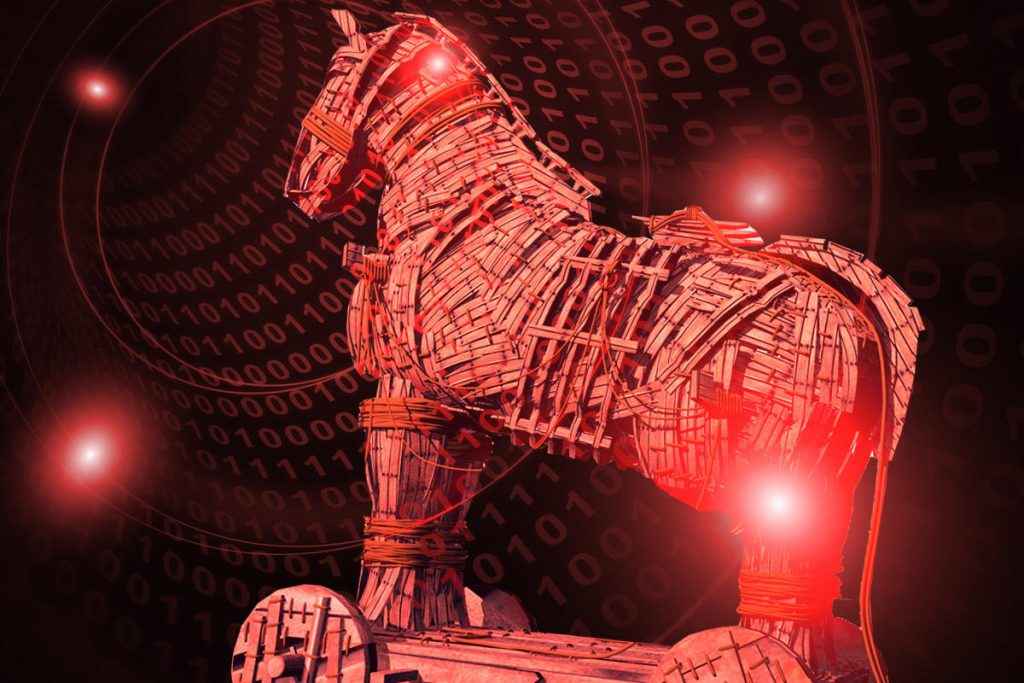
\includegraphics[width=1\linewidth]{Trojan.png}
    \caption{Wizualizacja konia trojańskiego jako metafory złośliwego oprogramowania. \cite{grafiki}}
    \label{fig:trojan}
\end{figure}
\newpage
\subsection{Przykład- Watykańczyk\index{Watykańczyk}}
\begin{itemize}
    \item \textbf{Pochodzenie:} Polska (ok. 2016 roku)
    \item \textbf{Typ:} Specyficzna forma złośliwego oprogramowania (tzw. joke program\index{joke program}) \cite{papiez}
    \item \textbf{Sposób działania:} Utrudniał korzystanie z komputera poprzez sekwencję zdarzeń.
    \item \textbf{Skutki infekcji:} Nie niszczył i nie kradł danych jego zadaniem było trollowanie użytkownika 
\end{itemize}
Film z demonstracją działania został opisany w Dodatku \ref{zal:watykanczyk}
\begin{figure}[!h]
        \centering
        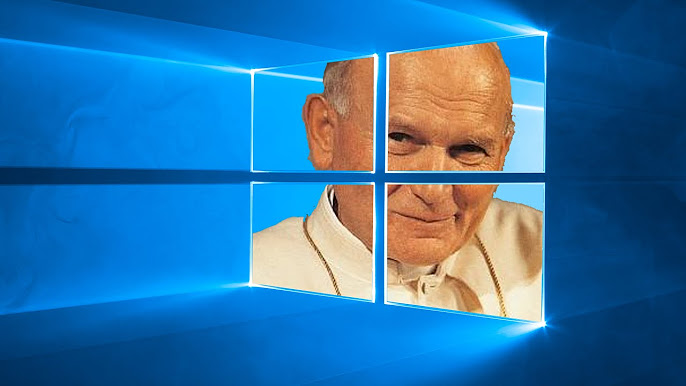
\includegraphics[width=1\linewidth]{papiez.png}
        \caption{Modyfikacja tapety systemu Windows charakterystyczna dla działania programu Watykańczyk. \cite{grafiki}}
        \label{fig:watykanczyk}
    \end{figure}
\newpage
\begin{figure}[!h]
        \centering
        
\includegraphics[width=1\linewidth]{dziekuje_za_uwage.png}
        \caption{Dziękuję za uwagę. \cite{grafiki}}
        \label{fig:slajd_końcowy}
    \end{figure}
    

\begin{thebibliography}{9}
    \bibitem{prezentacja} \textbf{Prezentacja:}\\ Cezary Kosowski,              \textit{\href{Informatyka_prezentacja.pptx}{Informatyka\_prezentacja.pptx}}.
    \bibitem{wirus} \textbf{Wirus komputerowy:}\\ \textit{\url{https://www.malwarebytes.com/pl/computer-virus}}       
    \bibitem{wirus_przyklad} \textbf{Przykład Wirusa:}\\ \textit{\url{https://www.blog.omegasoft.pl/czarnobyl-wirus-komputerowy/}}
    \bibitem{robak} \textbf{Robak sieciowy:}\\ \textit{\url{https://www.malwarebytes.com/pl/computer-worm}}
    \bibitem{robak_morris} \textbf{Robak Morrisa:}\\ \textit{\url{https://pl.wikipedia.org/wiki/Robak_Morrisa}}        \bibitem{ransomware} \textbf{Ransomware:}\\ \textit{\url{https://www.malwarebytes.com/pl/ransomware}}
    \bibitem{wannacry} \textbf{WannaCry:}\\ \textit{\url{https://www.malwarebytes.com/pl/wannacry}}
    \bibitem{trojan} \textbf{Trojan:}\\ \textit{\url{https://www.malwarebytes.com/pl/trojan}}
    \bibitem{papiez} \textbf{Watykańczyk:}\\ \textit{\url{https://www.instalki.pl/news/software/wirus-watykanczyk-jak-dzialal-2137/}}
    \bibitem{grafiki} \textbf{Grafiki:} \textit{Google grafika}, \textit{\url{https://gemini.google.com/app}} oraz \textit{archiwum prywatne}
\end{thebibliography}

\appendix
\chapter{Materiały dodatkowe}
\section{prezentacja}
Niniejszy dokument powstał na bazie prezentacji. Plik źródłowy w formacie programu PowerPoint znajduje się w katalogu głównym projektu i można go otworzyć klikając w poniższy link:
\href{Informatyka_prezentacja.pptx}{\textbf{Otwórz plik: Informatyka\_prezentacja.pptx}}

\section{Materiały wideo}
\label{zal:watykanczyk}
Dodatkowe materiały prezentujące działanie programu ,,Watykańczyk'' w środowisku wirtualnym:
\begin{itemize}
    \item Demonstracja infekcji --> \url{https://www.youtube.com/watch?v=V_twDHVXdNw&t=0s}
\end{itemize}
\printindex

\end{document}
